\documentclass[8pt]{beamer}
\usetheme{default} % Very simple theme
\usecolortheme{dove} % Minimalist grayscale colors
\setbeamertemplate{navigation symbols}{} % Remove navigation bar

% Define brand-like colors
\definecolor{myblue}{RGB}{0, 102, 204}    % Blue for standard blocks
\definecolor{mygreen}{RGB}{0, 153, 0}     % Green for example blocks
\definecolor{myred}{RGB}{204, 0, 0}       % Red for alert blocks
\definecolor{myorange}{RGB}{255, 128, 0} % For \emph

% Accent color for titles, bullets, etc.
\setbeamercolor{structure}{fg=myblue}

% Block colors
\setbeamercolor{block title}{bg=myblue, fg=white}
\setbeamercolor{block body}{bg=blue!5, fg=black}

\setbeamercolor{exampleblock title}{bg=mygreen, fg=white}
\setbeamercolor{exampleblock body}{bg=green!5, fg=black}

\setbeamercolor{alertblock title}{bg=myred, fg=white}
\setbeamercolor{alertblock body}{bg=red!5, fg=black}
\setbeamercolor{alerted text}{fg=myred}

% Optional: color for \example text
\setbeamercolor{example text}{fg=mygreen}

% Custom emph (orange text instead of italic)
\let\oldemph\emph
\renewcommand{\emph}[1]{\textcolor{myorange}{#1}}
\newcommand{\ve}[1]{\boldsymbol{#1}}

\usepackage{graphicx} % Package for images
\usepackage{amsmath} % Package for images
\graphicspath{{figs/}} % Path to your figures directory
\usepackage{array}  % For better column spacing
\usepackage{caption} % Required for \captionof
%\usepackage{enumitem}

% Title Information
\title{STOCHASTIC METHODS IN WATER RESOURCES}
\vspace{25pt}
\subtitle{Unit 5: Geostatistics \\ Lecture 17: Ordinary and block kriging}
\author{Luis Alejandro Morales, Ph.D.}
\institute{Universidad Nacional de Colombia \\ Department of Civil and Agriculture Engineering} %// }
%\date{\today}

\begin{document}

% Title Slide
\begin{frame}
    \titlepage
\end{frame}

%-------
% From Bierkens
\section{Spatial interpolation by kriging}
 \begin{frame}{Spatial interpolation by kriging}
     \begin{block}{Ordinary kriging}
    \end{block}
    \alert{Ordinary kriging} can be used if:
    \begin{enumerate}
        \item $Z(\mathbf{x})$ is a \emph{wide sense stationary random function} but the mean of $Z(\mathbf{x})$ is unknown, or
        \item $Z(\mathbf{x})$ is an intrinsic \emph{random function}.
    \end{enumerate}
    An intrinsic \emph{random function} has the following properties:
    \[
        E[Z(\mathbf{x}_2) - Z(\mathbf{x}_1)] = 0
    \]
    \[
        E[Z(\mathbf{x}_2) - Z(\mathbf{x}_1)]^2 = 2\gamma(\mathbf{x}_2 - \mathbf{x}_1) = 2 \gamma(\mathbf{h})
    \]

    The mean difference between the \emph{random variates} at any two locations is zero (i.e. \emph{constant mean}) and the  \emph{variance} of this difference is a function that only depends on the separation vector $\mathbf{h}$. The function $\gamma(\mathbf{h}) = \frac{1}{2} E[Z(\mathbf{x})-Z(\mathbf{x}+\mathbf{h})]^2 $ is the \emph{semivariogram}.

    The \emph{ordinary kriging predictor} is a weighted average of the surrounding observations
    \begin{equation}
        \hat{Z}(\mathbf{x}_0) = \sum_{i=1}^n \lambda_i Z(\mathbf{x}_i)
        \label{e714}
    \end{equation}
with $Z(\mathbf{x}_i)$ the values of $Z(\mathbf{x})$ at the observation locations (usually within a limited search neighbourhood). 
   \end{frame}

 \begin{frame}{Spatial interpolation by kriging}
     \begin{block}{Ordinary kriging}
    \end{block}
    As with the \emph{simple kriging} predictor, the equation~\ref{e714} must be unbiased
    \begin{equation}
    E[\hat{Z}(\mathbf{x}_0) - Z(\mathbf{x}_0)] =  E\left[ \sum_{i=1}^n \lambda_i Z(\mathbf{x}_i) -Z(\mathbf{x}_0) \right] =  \sum_{i=1}^n \lambda_i E[Z(\mathbf{x}_i)] - E[Z(\mathbf{x}_0)] = 0
        \label{e715}
    \end{equation}
As the unknown \emph{mean} is constant, i.e. $E[Z(\mathbf{x}_i)] = E[Z(\mathbf{x}_0)] \forall \mathbf{x}_i , \mathbf{x}_0$, we find the following \emph{unbiasedness constraint} for the $\lambda_i$
    \begin{equation}
        \sum_{i=1}^n \lambda_i = 1
        \label{e716}
    \end{equation}

    Apart from being unbiased we also want to have a predictor with a \emph{minimum variance} of the \emph{prediction error}. The \emph{error variance} for predictor (see equation~\ref{e714}) can be written in terms of the \emph{semivariance} as 

    \begin{equation}
        \begin{aligned}
            &var[\hat{Z}(\mathbf{x}_0) - Z(\mathbf{x}_0)] = E[\hat{Z}(\mathbf{x}_0) - Z(\mathbf{x}_0)]^2 = \\ 
            &-\sum_{i=1}^n \sum_{j=1}^n \lambda_i \lambda_j \gamma_Z (\mathbf{x}_i - \mathbf{x}_j) + 2\sum_{i=1}^n \lambda_i \gamma_Z (\mathbf{x}_i - \mathbf{x}_0)
        \end{aligned}
        \label{e717}
    \end{equation}
    We want to minimize the \emph{error variance} subject to the constraint given by equation~\ref{e716}. In other words, we want to find the set of values $\lambda_i, i=1,2,\cdots,n$  for which equation~\ref{e717} is minimum without violating constraint in equation~\ref{e716}. 
   \end{frame}

 \begin{frame}{Spatial interpolation by kriging}
     \begin{block}{Ordinary kriging}
    \end{block}
To find these, a mathematical trick is used. First the expression of the error variance is extended as follows
    \begin{equation}
        \begin{aligned}
            & E[\hat{Z}(\mathbf{x}_0) - Z(\mathbf{x}_0)]^2 = \\ 
            &\sum_{i=1}^n \sum_{j=1}^n \lambda_i \lambda_j \gamma_Z (\mathbf{x}_i - \mathbf{x}_j) + 2\sum_{i=1}^n \lambda_i \gamma_Z (\mathbf{x}_i - \mathbf{x}_0) - 2\nu\left[\sum_{i=1}^n \lambda_i - 1 \right] 
        \end{aligned}
        \label{e718}
    \end{equation}
    If the estimator is really \emph{unbiased}, nothing has happened to the \emph{error variance} as the added term is zero by definition. The dummy variable $\nu$ is called the \alert{Lagrange multiplier}. It can be shown that if we find the set of $\lambda_i, i=1,2,\cdots, n$ and the value of $\nu$ for which equation~\ref{e718} has its minimum value, we have also have the set of $\lambda_i (\mathbf{x}_0), i=1,2,\cdots,n$ for which the \emph{error variance} of the \emph{ordinary kriging predictor} is minimal, while at the same time $\sum \lambda_i =1$. As with \emph{simple kriging}, the minimum value is found by partial differentiation of equation~\ref{e718} with respect to $\lambda_i, i=1,2,\cdots, n$  and $\nu$ and equating the partial derivatives to zero. This results in the following system of $(n + 1)$ linear equations

    \begin{equation}
        \sum_{j=1}^n \lambda_j \gamma_Z(\mathbf{x}_i - \mathbf{x}_j ) +  \nu = \gamma_Z (\mathbf{x}_i - \mathbf{x}_0) \quad \quad \sum_{i=1}^n \lambda_i = 1 \quad \quad i=1,\cdots,n
        \label{e719}
    \end{equation}
    Using the \emph{Lagrange multiplier}, the value for the (minimum) variance of the \emph{prediction error} can be conveniently written as
    \vspace{-5pt}
    \begin{equation}
        var[\hat{Z}(\mathbf{x}_0) - Z(\mathbf{x}_0)] = \sum_{i=1}^n \lambda_i \gamma_Z (\mathbf{x}_i - \mathbf{x}_0) + \nu 
        \label{e720}
    \end{equation}
   \end{frame}

 \begin{frame}{Spatial interpolation by kriging}
     \begin{block}{Ordinary kriging}
    \end{block}
    A unique solution of the system in equation~\ref{e719} and a positive \emph{kriging variance} is only ensured if the \emph{semivariogram function} is \emph{conditionally non-negative definite}. This means that for all possible $\mathbf{x}_i, \cdots, \mathbf{x}_n \in  \Re  (N=1,2\ or\ 3)$ and for all $\lambda_1, \cdots, \lambda_n \in \Re$ such that $\sum_i \lambda_i =1$, the following inequality must hold
    \vspace{-5pt}
    \begin{equation}
        -\sum_{i=1}^n \sum_{j=1}^n \lambda_i \lambda_j \gamma_Z (\mathbf{x}_i - \mathbf{x}_j) \geq 0
        \label{e721}
    \end{equation}
    This is ensured if one of the permissible \emph{semivariogram models} in the table below is fitted to the \emph{experimental semivariogram} data.
    \begin{center}
  \begin{tabular}{|l|c|}
    Spherical model         & $ \gamma (h) = \left\{ \begin{array}{l}  c \left[ \frac{3}{2}\left(\frac{h}{a}\right) - \frac{1}{2}\left(\frac{h}{a}\right)^3 \right]   \text{, if } h\leq a  \\ c  \text{, if } h > a \end{array} \right. $ \\ 
    Exponential model & $\gamma (h) = c \left[1- e^{-h/a} \right]$ \\ 
    Gaussian model         & $\gamma (h) =  c\left[1- e^{-h^2 / a^2} \right] $ \\ 
    Nugget model &  $ \gamma (h) = \left\{ \begin{array}{l}  0 \text{, if } h=0  \\ 1 = \text{, if } h>0 \end{array} \right. $ \\ 
    Power model & $\gamma (h) = ch^\omega \text{, if } 0<\omega<2 $
  \end{tabular}
    \end{center}
    where $h$ denotes the length of the lag vector $\mathbf{h}$.

    Note that the \emph{exponential and nugget} models are also permissible in cases the \emph{random function} is \emph{wide sense stationary}. The \emph{power model}, which does not reach a \emph{sill} (value at which the semivariogram levels off, meaning the semivariance stops increasing with distance) can be used in case of an intrinsic \emph{random function} but not in case of a wide sense stationary \emph{random function}.
 
   \end{frame}

 \begin{frame}{Spatial interpolation by kriging}
     \begin{block}{Ordinary kriging}
    \end{block}
    \begin{itemize}
        \item The unknown \emph{mean} $\mu_Z$ and the \emph{langrange multiplier} $\nu$ require some further explanation. If all the data are used to obtain predictions at every location, at all locations the same unknown \emph{mean} $\mu_Z$ is implicitly estimated by the \emph{ordinary kriging predictor}.
        \item The \emph{Lagrange multiplier} represents the additional uncertainty that is added to the \emph{kriging prediction} by the fact that the \emph{mean} is unknown and must be estimated.
        \item Therefore, if the \emph{random function} is \emph{wide sense stationary}, the \emph{variance} of the \emph{prediction error} for \emph{ordinary kriging} is larger than that for \emph{simple kriging}, the difference being the \emph{Lagrange multiplier}.
        \item This can be deduced from substituting in equation~\ref{e720} $\gamma_Z (\mathbf{h}) = \sigma_Z^2 - C_Z(\mathbf{h})$ and taking into account that $\sum_i \lambda_i = 1$. This means that, whenever the \emph{mean} is not exactly known and has to be estimated from the data it is better to use \emph{ordinary kriging}, so that the added uncertainty about the \emph{mean} is taken into account.
        \item Even in \emph{simple kriging} one rarely uses all data to obtain \emph{kriging predictions}. Usually only a limited number of data close to the \emph{prediction location} are used. This is to avoid that the \emph{kriging systems} become too large and the mapping too slow.
        \item The most common way of selecting data is to center an \emph{area} or \emph{volume} at the \emph{prediction location} $\mathbf{x}_0$ . Usually the \emph{radius} is taken about the size of the \emph{variogram range}. A limited number of data points that fall within the \emph{search area} are retained for the \emph{kriging prediction}.
    \end{itemize}
   \end{frame}
 
 \begin{frame}{Spatial interpolation by kriging}
     \begin{block}{Ordinary kriging}
    \end{block}
    \begin{itemize}
        \item This means that the number of data locations becomes a function of the prediction location: $n \equiv n(\mathbf{x}_0)$. Also, if \emph{ordinary kriging} is used, a local mean is implicitly estimated that changes with $\mathbf{x}_0$. So we have $\mu \equiv \mu (\mathbf{x}_0)$  and $\nu \equiv \nu(\mathbf{x}_0)$ footnote .
        \item This shows that, apart from correcting for the uncertainty in the \emph{mean} and being able to cope with a weaker form of \emph{stationarity}, \emph{ordinary kriging} has a third advantage when compared to \emph{simple kriging}: even though the intrinsic hypothesis assumes that the \emph{mean} is constant, using \emph{ordinary kriging} with a search neighbourhood enables one to correct for \emph{local deviations} in the \emph{mean}.
        \item This makes the \emph{ordinary kriging predictor} more robust to \emph{trends} in the data than the \emph{simple kriging predictor}.

    \end{itemize}
   \end{frame}

 \begin{frame}{Spatial interpolation by kriging}
    \begin{block}{Ordinary kriging: practical application}
    \end{block}
    \begin{enumerate}
        \item Estimate the \emph{semivariogram}
        \item Fit a permissible \emph{semivariogram model}
        \item For every node on the grid repeat:
    \begin{enumerate}
        \item Solve the \emph{kriging equations}: Using the fitted \emph{semivariogram model} $\gamma_Z (\mathbf{h})$ in the $n+1$ linear equations~\ref{e719} yields, after solving them, the \emph{kriging weights} $\lambda_i,\ i=1,2,\cdots,n$ and the \emph{Lagrange multiplier} $\nu$.
        \item Predict the value $Z(\mathbf{x}_0)$: With the $\lambda_i$ , the observed values $z(\mathbf{x}_i)$ (usually within the search neighbourhood) in equation~\ref{e714} the unknown value of $Z(\mathbf{x}_0)$ is predicted.
        \item Calculate the \emph{variance} of the \emph{prediction error}: Using $\lambda_i$, $\gamma_z (\mathbf{h})$ and $\nu$ the \emph{variance} of the \emph{prediction error} is calculated with equation~\ref{e720}.

    \end{enumerate}
    \end{enumerate}
    The figure shows the \emph{ordinary kriging prediction} and the \emph{ordinary kriging variance}.

            \begin{center}
            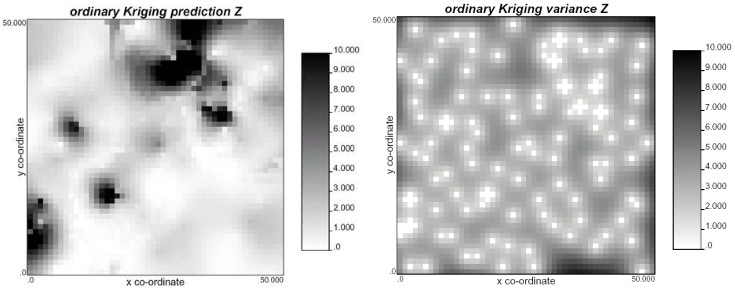
\includegraphics[width=0.9\linewidth]{fiBi710.png}  % from Bierk
            \end{center}
   \end{frame}
 
 \begin{frame}{Spatial interpolation by kriging}
     \begin{block}{Block kriging}
    \end{block}
    \begin{itemize}
        \item Up to known we have been concerned with predicting the values of attributes at the same  support (averaging volume) as the observations, usually point support. However, in many cases one may be interested in the mean value of the attribute for some area or volume much larger than the support of the observations.
        \item For instance, one may be interested in the \emph{average porosity} of a model block that is used in a \emph{numerical groundwater model}, or the \emph{average precipitation} of a catchment. These average quantities can be predicted using \alert{block kriging}.
        \item The term \emph{block kriging} is used as opposed to \emph{point kriging} or \emph{punctual kriging} where attributes are predicted at the same support as the observations. Any form of \emph{kriging} has a \emph{point} form and a \emph{block} form.
        \item So, there is \emph{simple point kriging} and \emph{simple block kriging} and \emph{ordinary point kriging} and \emph{ordinary block kriging}. Usually, the term \emph{point} is omitted and the term \emph{block} is added only if the \emph{block kriging} form is used.
    \end{itemize}
   \end{frame}

  \begin{frame}{Spatial interpolation by kriging}
     \begin{block}{Block kriging}
    \end{block}
    Consider the problem of predicting the \emph{mean} $Z$ of the attribute $z$ that varies with spatial coordinate $\mathbf{x}$ for some \emph{area} or \emph{volume} $D$ with size $|D|$ (length, area or volume)
    \begin{equation}
        \bar{Z} = \frac{1}{|D|} \int_{\mathbf{x} \in D} Z(\mathbf{x}) d\mathbf{x}
        \label{e722}
    \end{equation}
In case $D$ is a block in three dimensions with upper an lower boundaries boundaries $x_l$, $y_l$, $z_l$, $x_u$, $y_u$, $z_u$ the spatial integral in equation~\ref{e722} stands for

    \begin{equation}
         \frac{1}{|D|} \int_{\mathbf{x} \in D} Z(\mathbf{x}) d\mathbf{x} = \frac{1}{|x_u - x_l| |y_u - y_l| |z_u - z_l|} \int_{z_l}^{z_u}\int_{y_l}^{y_u}\int_{x_l}^{x_u} Z(s_1, s_2, s_3 ) ds_1 ds_2 ds_3
        \label{e723}
    \end{equation}

\begin{minipage}[]{0.48\textwidth}
Of course, the block $D$ can be of any form, in which case a more complicated spatial integral is used. The figure  shows how to predict the mean value of $Z$ of some irregular 2D area $D$.
\end{minipage}
\hfill
\begin{minipage}[]{0.48\textwidth}
            \begin{center}
            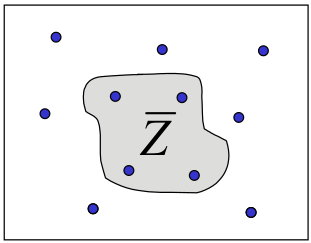
\includegraphics[width=0.9\linewidth]{fiBi711.png}  % from Bierk
            \end{center}
\end{minipage}

   \end{frame}
    
  \begin{frame}{Spatial interpolation by kriging}
     \begin{block}{Block kriging}
    \end{block}
    Similar to \emph{point kriging}, the unknown value of $\bar{Z}$ can be predicted as linear combination of the observations by assuming that the predictant and the observations are partial realizations of a \emph{random function}. So, the \emph{ordinary bock kriging predictor} becomes
    \begin{equation}
        \hat{\bar{Z}} = \sum_{i=1}^n \lambda_i Z(\mathbf{x}_i)
        \label{e724}
    \end{equation}
    where the \emph{block kriging weights} $\lambda_i$ are determined such that $\hat{\bar{Z}}$ is unbiased and the prediction variance $var\left[\hat{\bar{Z}} - \bar{Z} \right]$ is minimal. This is achieved by solving the $\lambda_i$  from the \emph{ordinary block kriging system}

    \begin{equation}
        \sum_{j=1}^n \lambda_j \gamma_Z (\mathbf{x}_i - \mathbf{x}_j) + \nu = \gamma_Z (\mathbf{x}_i, D) \quad \quad \sum_{i=1}^n \lambda_i = 1 \quad \quad i=1,2,\cdots,n 
        \label{e725}
    \end{equation}
    It can be seen that the \emph{ordinary block kriging system} looks almost the same as the \emph{ordinary (point) kriging system}, except for the term on the right hand side which is the average \emph{semivariance} between a location $\mathbf{x}_i$ and all the locations inside the area of interest $D$
    \vspace{-5pt}
    \begin{equation}
        \gamma_Z (\mathbf{x}_i, D) = \frac{1}{|D|} \int_{\mathbf{x} \in D} \gamma_Z (\mathbf{x}_i - \mathbf{x}) d\mathbf{x}
        \label{e726}
    \end{equation}
   \end{frame}

  \begin{frame}{Spatial interpolation by kriging}
     \begin{block}{Block kriging}
    \end{block}

    When building the \emph{block kriging system}, the integral in equation~\ref{e726} is usually not solved. Instead, it is approximated by
    \begin{enumerate}
        \item discretizing the area of interest in a limited number of points. 
        \item the \emph{semivariances} are calculated between the observation location and the $N$ points $\mathbf{x}_j$ discretizing $D$ (see left figure).
            \begin{center}
            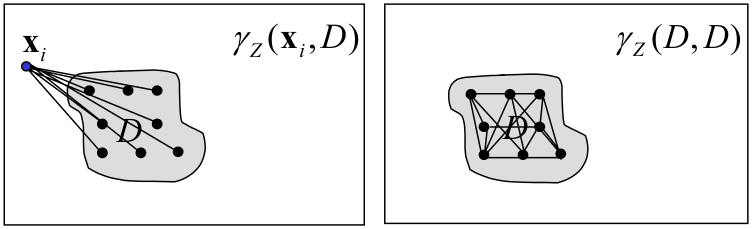
\includegraphics[width=\linewidth]{fiBi712.png}  % from Bierk
            \end{center}
        \item the \emph{average semivariance} is approximated by averaging these \emph{semivariances} as:
    \begin{equation}
        \gamma_Z (\mathbf{x}_i, D) \simeq \frac{1}{N} \sum_{j=1}^N \gamma_Z (\mathbf{x}_i - \mathbf{x}_j) 
        \label{e727}
    \end{equation}
    \end{enumerate}
   \end{frame}

  \begin{frame}{Spatial interpolation by kriging}
     \begin{block}{Block kriging}
    \end{block}
The variance of the prediction error is given by
    \begin{equation}
        var [\hat{\bar{Z}} - \bar{Z} ] = E[\hat{\bar{Z}} - \bar{Z}]^2 = \sum_{i=1}^n \lambda_i \gamma_Z (\mathbf{x}_i, D ) + \nu - \gamma_Z (D,D) 
        \label{e728}
    \end{equation}
    where $\gamma_Z(D,D)$ is the \emph{average semivariance} within the area $D$, i.e. the \emph{average semivariance} between all locations with $D$:

    \begin{equation}
        \gamma_Z (D,D) = \frac{1}{|D|^2} \int_{\mathbf{x}_2 \in D} \int_{\mathbf{x}_1 \in D} \gamma(\mathbf{x}_1 - \mathbf{x}_2 ) d\mathbf{x}_1 d\mathbf{x}_2
        \label{e729}
    \end{equation}
    which in practice is approximated by $N$ points $\mathbf{x}_i$ discretizing $D$ as (see right figure above)
    \begin{equation}
        \gamma_Z (D,D) = \frac{1}{N^2} \sum_{i=1}^N \sum_{j=1}^N \gamma(\mathbf{x}_i - \mathbf{x}_j ) 
        \label{e730}
    \end{equation}
   \end{frame}

  \begin{frame}{Spatial interpolation by kriging}
     \begin{block}{Block kriging}
    \end{block}
    The figure below shows the result of \emph{block kriging} with \emph{block sizes} of 5x5 units.
            \begin{center}
            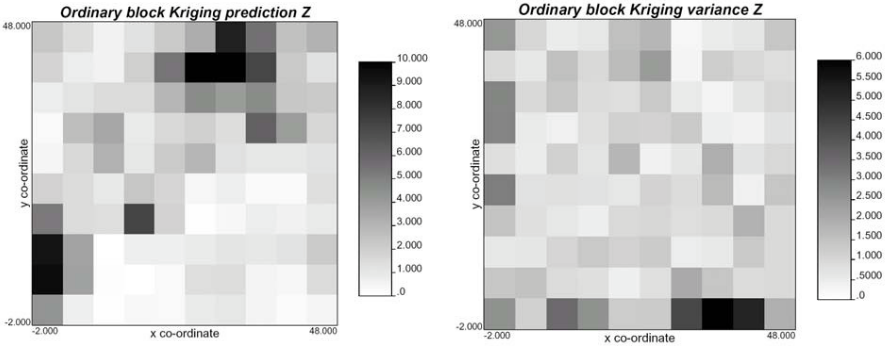
\includegraphics[width=\linewidth]{fiBi713.png}  % from Bierk
            \end{center}
     \begin{itemize}
         \item Here we have given the equations for ordinary block kriging.
         \item The \emph{simple block kriging} equations can be deduced in a similar manner from the \emph{simple kriging equations}  by replacing the \emph{covariance} on the right hand side of the equation by the \emph{point-block covariance} $C_Z (\mathbf{x}_i, D)$.
         \item In the \emph{prediction error variance}, $\sigma_Z^2$ is replaced by the within block variance $C_Z (D,D)$ (the average covariance of points within $D$) and $C_Z (\mathbf{x}_i - \mathbf{x}_0)$ by $C_Z (\mathbf{x}_i, D)$.
         \item The \emph{point-block covariance} and the \emph{within block covariance} are defined as in equations~\ref{e726} and ~\ref{e729} with $\gamma_Z(\mathbf{x}_1 - \mathbf{x}_2)$ replaced by $C_Z (\mathbf{x}_1 - \mathbf{x}_2)$.
     \end{itemize}
   \end{frame}

%   \begin{frame}{Spatial interpolation by kriging}
     % \begin{block}{Block kriging}
    % \end{block}
     % \begin{itemize}
         % \item Equation~\ref{e730} can be used to map the \emph{probability of exceeding} this threshold, given the concentrations found at the observation locations.
         % \item In a \emph{groundwater solute transport problem}, instead of delineating a \emph{single plume} based upon some predicted value, \emph{several alternative plumes} can be delineated, depending on which probability contour is taken as its boundary.
         % \item This way, both the \emph{observed concentration} values as well as the \emph{local uncertainty} are taken into account when mapping the plume. 
         % \item Also, the \emph{risk} of not treating \emph{hazardous groundwater} can be weighted against the \emph{costs of remediation}. For instance, if the risk of not treating \emph{hazardous groundwater} should be smaller than 5\%, all the water within the 0.05 contour should be treated.
         % \item Obsviously this results in much higher costs then if, for instance, a 10\% \emph{risk} is deemed acceptable.
     % \end{itemize}

   % \end{frame}

\end{document}



